\section{Experimental Evaluation}

In this section, we will empirically evaluate the performance of known approximation algorithms for item pricing and bundle pricing. Our goal is to understand the behavior of the algorithms on practical \texttt{SQL} queries over real world datasets. We will first describe our experimental setup, followed by the algorithms that we use and various knobs that we can control to create different instances of the hypergraph instances. 

\subsection{Experimental setup}

We perform all our experiments on $2.2$ GHz processor machine with $4$ cores and $16$ GB main memory running OS X $10.10.5$. We use \texttt{MySQL} as our underlying database for query processing and evaluation. Our implementation is written in \textsc{Python} as an enhancement in \textsc{Qirana} prototype system. \textsc{Qirana} generates random neighbors of a database over which query pricing is performed. The advantage of using neighbors is that we can succinctly represent the neighbor without storing the new database, i.e, we can represent the neighbor by storing only the \emph{update query} that generates the neighbor. \textsc{Qirana} generates two types of neighbors: $(i)$ row update; $(ii)$ swap update. A row update changes one attribute of a single tuple and replaces the attribute value with a different value from the specified domain of the particular attribute. For example,  the following row update modifies the \textsf{User.gender} value of the tuple with key $1$ to f to create a neighboring instance of $D$: 

\begin{center}
	\texttt{UPDATE User SET gender = ’f ’ WHERE uid = 1;}
\end{center}

A swap update on the other hand, exchanges the attribute values of $2$ random tuples in a single relation. For example, the following swap update sets
\textsf{User.age} $= 19$ for the tuple with key $1$ and \textsf{User.age} $= 25$ for
the tuple with key $4$:

\begin{center}
\texttt{UPDATE User SET age = 19 WHERE uid = 1;} 

\texttt{UPDATE User SET age = 25 WHERE uid = 4;}
\end{center}

Both row and swap updates generate a neighboring database that is different from $D$. The set of all neighboring databases is called as the \emph{support set} $\mS$. Observe that any \texttt{SQL} query can be expressed as a subset of $\mS$ and vice-versa. More formally,

\begin{proposition}
	Consider the underlying database $D$ and support set $\mS$. Then,
	\begin{enumerate}
		\item Any query $Q$ can be expressed by a unique set $T \subseteq \mS$ such that $T = \{ D' \in \mS \mid Q(D') \neq Q(D)\}$
		\item For any subset $T \subseteq \mS$, there exists a conjunctive query $Q$ such that $T = \{ D' \in \mS \mid Q(D') \neq Q(D)\}$
	\end{enumerate} 
\end{proposition}	

In our framework, given a workload of queries $Q_1, \dots, Q_k$, we define a matrix $M$ of size $k \times |\mS|$ that is initialized as follows, 

\begin{equation}
M[i][j]=\begin{cases}
1, & \text{if $Q_i(D) \neq Q_i(D')$ where $D'$ is the $j^{th}$ neighbor in $\mS$}.\\
0, & \text{otherwise}.
\end{cases}
\end{equation}

Thus, each row in matrix $M$ represents the \emph{disagreement} vector for a query $Q_i$ and can be viewed as a hyperedge where the set of vertices is $\mS$. In other words, matrix $M$ represents a hypergraph $H = (V, E)$ where $V = \mS$ and $E = \{ D' \mid M[i][D'] = 1\}$ for each query $Q_i$ in the workload. Additionally, for each query $Q_i$, we are given a valuation $v_i$ that represents the price a customer is willing to pay for the query. Recall that since our customer is a single minded buyer, we can make the sale only if price $p(Q_i) \leq v_i$. In the following, we will use query and hyperedge interchangeably to simplify the exposition. Without loss of generality, we will also assume that every hyperedge has exactly one customer who wants to purchase it. 

\subsection{Approximation Algorithms}

In this section, we will describe the pricing functions that we consider and the approximation algorithms that can be applied. We will consider two types of pricing schemes in our experiments: $(i)$ uniform bundle pricing; $(ii)$ item pricing. 

\smallskip
\introparagraph{Uniform Bundle Pricing} In this pricing scheme, the algorithm sells every hyperedge at a fixed price $p'$. Then, if the buyer has valuation $v_e \geq p'$, the hyperedge (and thus, the query corresponding to the hyperedge) can be sold. Uniform bundle pricing is very attractive as a pricing scheme for the following reasons, 

\begin{enumerate}
	\item Since all bundles are sold at a fixed take-it or leave-it price, it is a monotone and subadditive pricing function by definition
	\item Finding the right fixed price $p'$ can be done in time  $O(|E|^{2})$
	\item It does not depend on the size of the hyperedge, i.e, even if the hyperedge is empty, we can still sell the hyperedge
\end{enumerate}

However it also has downsides associated with it. First, the pricing scheme is insensitive to the output of the queries (and thus, their information content). Indeed, if all queries are sold at a fixed price, we ignore the actual content of the queries itself \footnote{One can argue that the value of the information content is encoded in the price that customers are willing to pay. This is only true if the buyers know the their valuation function exactly. In general, we want to use pricing functions that are sensitive to the hyperedge structure}. Second, we cannot encode history awareness in the uniform bundle prices. As the buyer purchases more hyperedges over time, we do not want to overcharge the buyer for information that has already been purchased. \shaleen{add an example here}. History awareness is easy to achieve via item pricing but if the pricing function is uniform, we will overcharge the buyer whenever there is overlap between two hyperedges that he/she wants to buy.

\begin{algorithm}[!htp]
	\SetCommentSty{textsf}
	\DontPrintSemicolon 
	\SetKwFunction{proc}{\textsf{eval}}
	\SetKw{KwGoTo}{go to}	
	\SetKwData{maxsum}{maxrev}
	\SetKwData{fixedprice}{fixedprice}
	\SetKwData{sum}{rev}
	\SetKwInOut{Input}{\textsc{input}}\SetKwInOut{Output}{\textsc{output}}
	%
	\Input{Hypergraph $H = (V, E)$ and valuation $v_e, e \in E$}
	\Output{Uniform price $p$}
	\BlankLine
	%
	$\maxsum \leftarrow 0, \fixedprice \leftarrow 0$ \\
	\For{$e \in E$}{
		$p \leftarrow v_e, sum \leftarrow 0$ \\
			\For{$e \in E$}{
				\If{$v_e \geq p$}{
					 $\sum \leftarrow \sum + p$ 
				 }
			}
		\If{$\sum > \maxsum$}{
			$\maxsum \leftarrow \sum, \fixedprice \leftarrow p$
		}
	}

	\KwRet{$\fixedprice$}
	\caption{Find revenue maximizing uniform bundle price}
	\label{algo:uniformbundleprice}
\end{algorithm}

Algorithm~\ref{algo:uniformbundleprice} shows how to find the revenue maximizing uniform bundle price which gives an $O(\log |E|)$ approximation where $v_{\max}, v_{\min}$ are the largest and smallest valuations for any hyperedge respectively.

\smallskip
\introparagraph{Item Pricing} In this pricing scheme, the algorithm will assign a weight to each vertex in the hypergraph. Then, the price of any hyperedge $e$ is given by $p(e) = \sum_{v : v \in e} w_v$. Item pricing is a natural fit for the query pricing framework since it allows for maintaining history of query purchases and is sensitive to the information content of the query. However, unlike uniform bundle pricing, we need to ensure that $\mS$ is big enough so that queries have a non-zero hyperedge size. If any query has no disagreement, then item pricing will assign a zero price to the query.

In our experiments, we use an optimization in $O(\log |V| + \log |E|)$-approximation algorithm given by~\cite{guruswami2005profit}. We consider all candidate uniform item prices $q_e = \frac{v_e}{|E|}$. Then, the algorithm will identify the set of hyperedges that can be sold by using $w_v = q_e$ for all vertices. Once we identify the subset of hyperedges that can be sold, we relax the uniform item pricing requirement and refine the weights by running a linear program. The final item weights are the ones that maximize the revenue. Algorithm~\ref{algo:itempricingbase} shows the detailed steps.

The second item pricing algorithm we consider is $O(\log B)$-approximation algorithm given by ~\cite{}. Although this algorithm was presented in the context of item pricing with limited supply, it readily extends to the unlimited supply setting.

\begin{algorithm}[!htp]
	\SetCommentSty{textsf}
	\DontPrintSemicolon 
	\SetKwFunction{proc}{\textsf{eval}}
	\SetKw{KwGoTo}{go to}	
	\SetKwData{maxsum}{maxrev}
	\SetKwData{fixedprice}{fixedprice}
	\SetKwData{temp}{temp}	
	\SetKwInOut{Input}{\textsc{input}}\SetKwInOut{Output}{\textsc{output}}
	%
	\Input{Hypergraph $H = (V, E)$ and valuation $v_e, e \in E$}
	\Output{Item weights $o$}
	\BlankLine
	%
	$\maxsum \leftarrow 0, \fixedprice \leftarrow 0, t$ \\
	\For{$e \in E$}{
		$q \leftarrow \frac{v_e}{|E|}, E' = \emptyset, w_v = \langle 0, \dots, 0 \rangle$ \\
		\For{$e \in E$}{
			\If{$v_e \geq |E| \cdot q$}{
				$E' \leftarrow E' \cup e$ 
			}
		}
		
		$\temp \leftarrow $maximize  $\sum_{e \in E'} w_v \cdot M[e]$ \\
		subject to \\
		$w_v \cdot M[e] \leq w_e$ for all $e \in E'$ \\
		$w_v \geq 0$
		
		\If{$\temp > \maxsum$}{$\maxsum \leftarrow \temp, t \leftarrow w_v$}
	}
	\KwRet{$t$}
	\caption{Find revenue maximizing uniform bundle price}
	\label{algo:itempricingbase}
\end{algorithm}

\subsection{Experiment Results}

Our first set of experiments is to understand how the approximation algorithms behave on real world queries. The first dataset we use is the $\texttt{\bfseries world}$ dataset, a popular database provided for software developers. It consists of $3$ relations: $\texttt{\bfseries Country}$,$\texttt{\bfseries CountryLanguage}$ and $\texttt{\bfseries City}$ which contain $5000$ tuples and $21$ attributes. We construct a support set of size $15000$ by randomly choosing neighboring databases. The query workload consists of $466$ queries containing selection, projections and join queries with aggregations. We construct the workload by generating changing the predicates in queries. The list of all queries is present in the appendix.

In order to compare different algorithms we use two upper bounds: $(i)$ sum of valuations, and $(ii)$ an upper bound on the optimal subadditive valuation. We find an upper bound on the optimal subadditive valuations by computing a linear program whose constraints encode the bundle arbitrage conditions. Since the number of constraints can be exponential in the number of hyperedges, we optimize by greedily adding constraints for bundles with largest valuations and finding a set of bundles that cover the hyperedge with small valuations. \shaleen{add example}.

\begin{figure*}[t]
	
	\begin{subfigure}{0.45\textwidth} 
		\hspace{-20mm}
		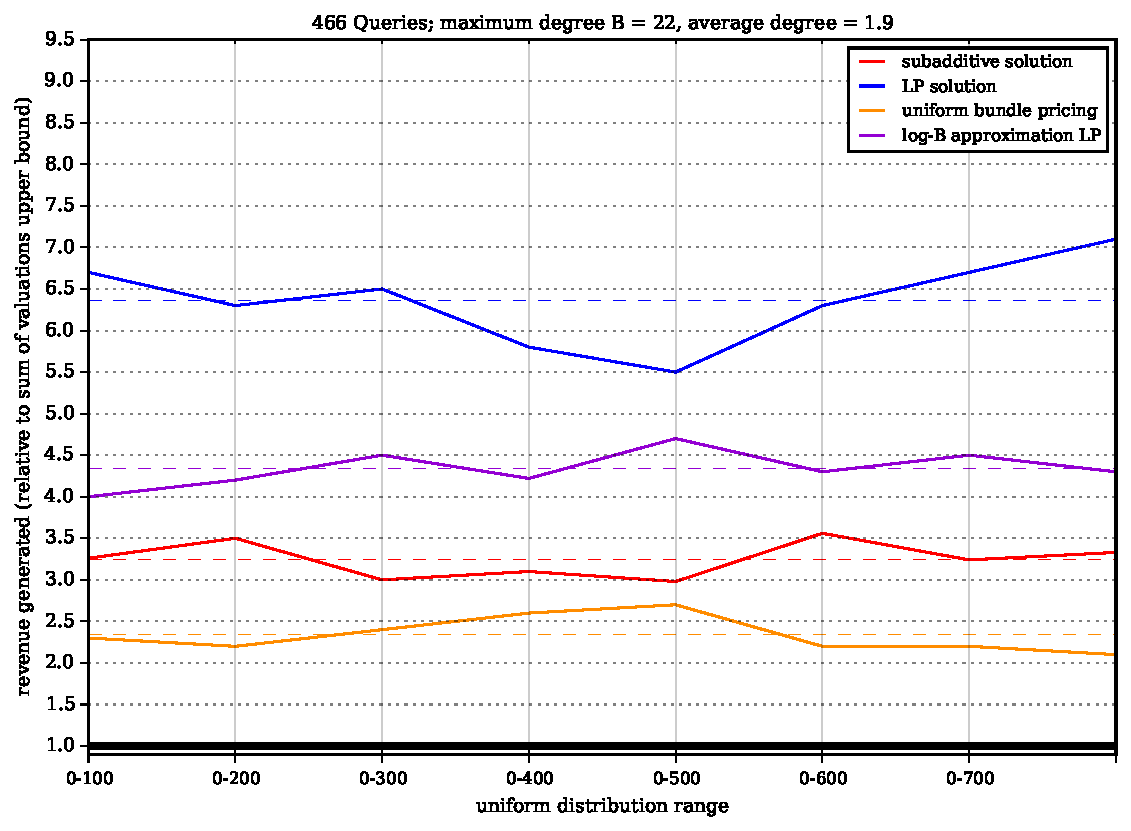
\includegraphics[scale=0.40]{uniformallapproxrealworkload.pdf}
		\caption{Algorithm performance - uniform valuations} \label{fig:uniformapprox}
	\end{subfigure} 
	\begin{subfigure}{0.45\textwidth} 
		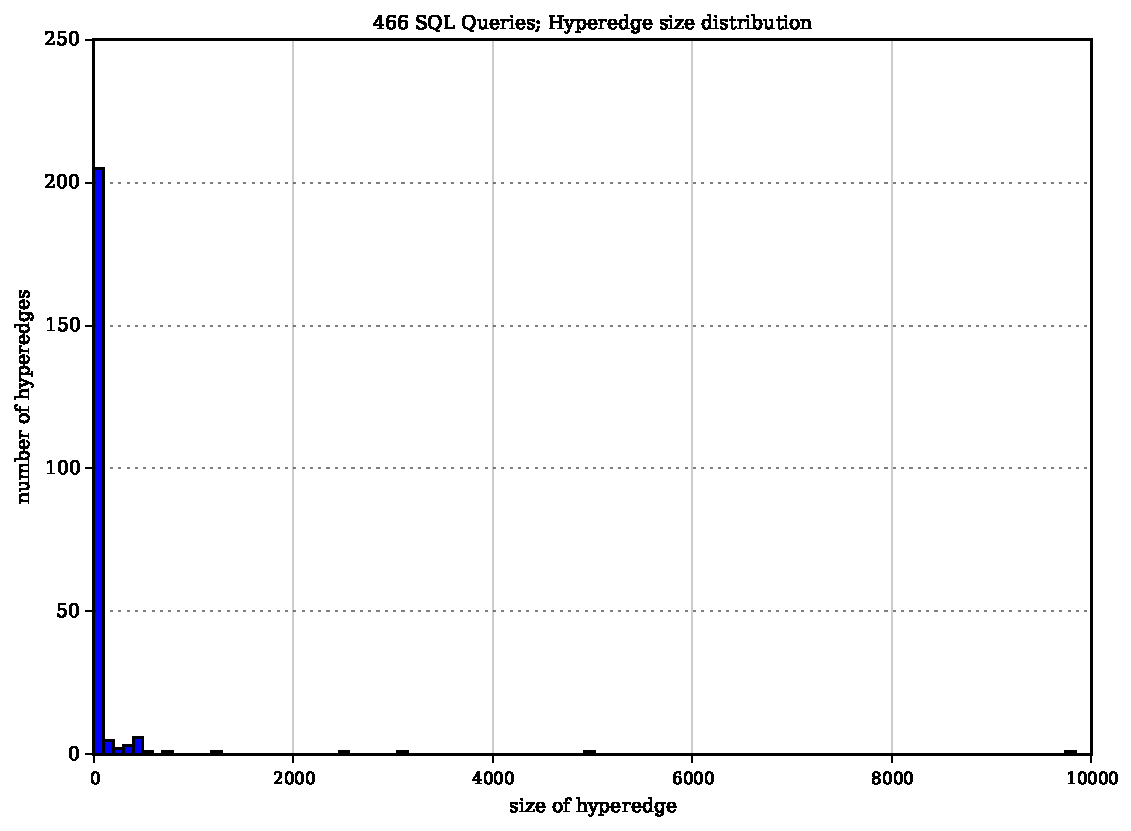
\includegraphics[scale=0.40]{histogramhyperedgesize.pdf}
		\caption{Hyperedge size histogram} \label{fig:histogramrealqueries}
	\end{subfigure} 
	\caption{Sampling valuations from uniform distribution}
\end{figure*}
\smallskip
\introparagraph{Sampling from uniform distribution} In our first experiment, we sample valuations from the uniform distribution. Figure~\ref{fig:uniformapprox} shows the performance of all algorithms. The first observation is that uniform bundle pricing outperforms all other algorithms. This is because bundle pricing does not depend on the hyperedge size or structure. For the given query workload, most hyperedges have size between $0$ to $1000$. As we will see later, for bigger sized hyperedges, item pricing performs better.

\begin{figure*}[t]
	
	\begin{subfigure}{0.45\textwidth} 
		\hspace{-20mm}
		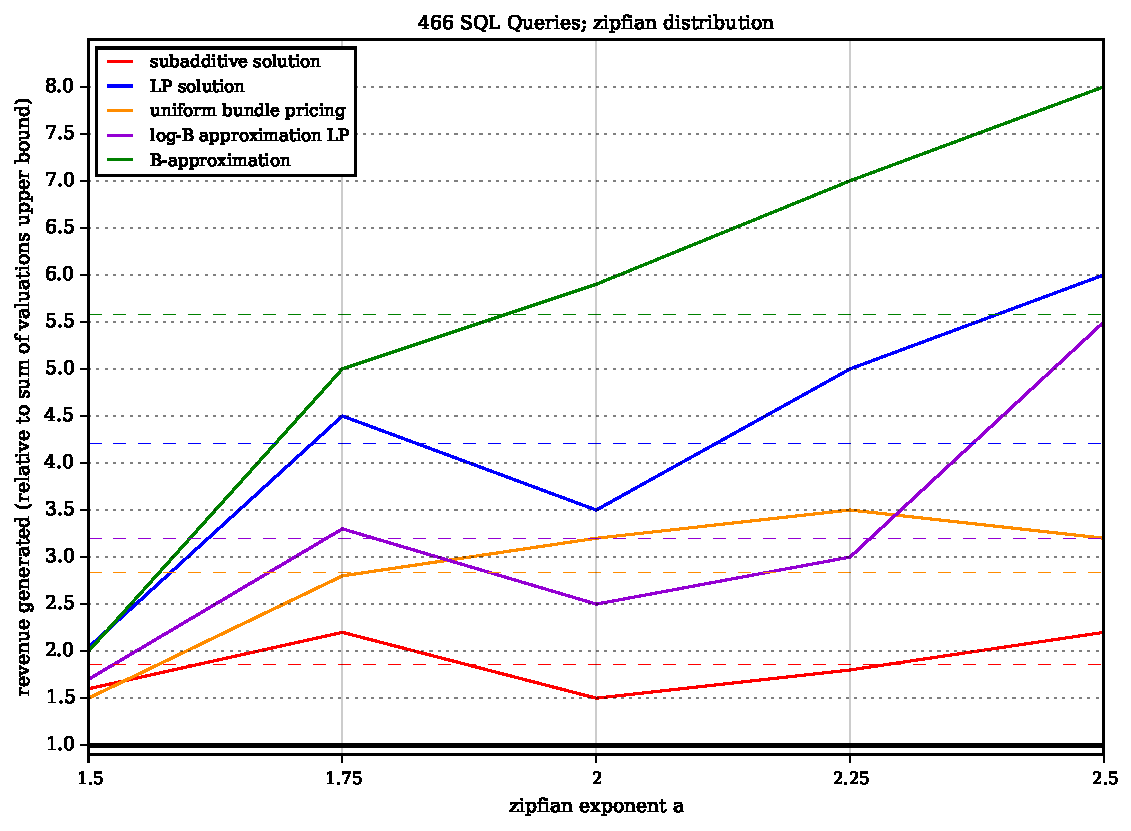
\includegraphics[scale=0.40]{zipfianallapproxrealworkload.pdf}
		\caption{Algorithm performance - zipfian distribution} \label{fig:zipfianapprox}
	\end{subfigure} 
	\begin{subfigure}{0.45\textwidth} 
		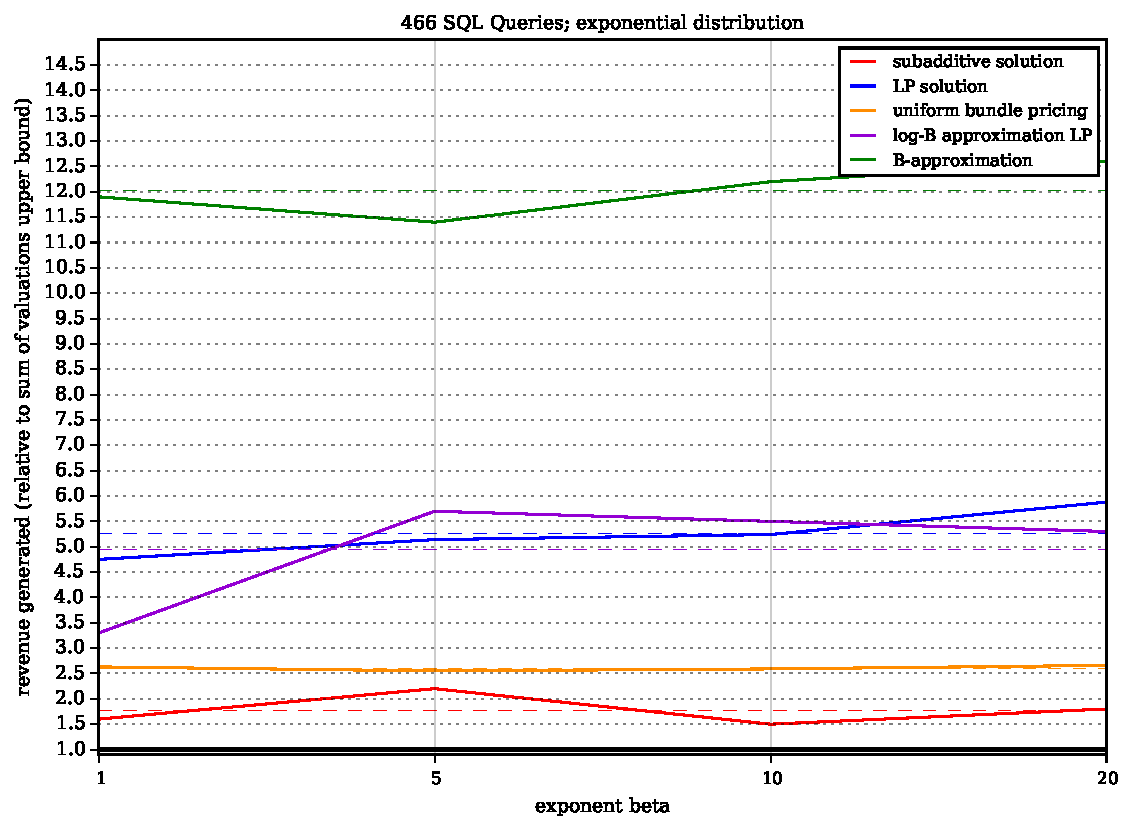
\includegraphics[scale=0.40]{exponentialallapproxrealworkload.pdf}
		\caption{Algorithm performance - exponential distribution} \label{fig:exponentialapprox}
	\end{subfigure} 
	\caption{Sampling valuations from zipfian and exponential distribution}
\end{figure*}

\smallskip
\introparagraph{Other distributions} Figure~\ref{fig:zipfianapprox} and~\ref{fig:exponentialapprox} perform the same experiment but sample valuation for hyperedges from zipfian and exponential distributions. Uniform bundle pricing is again better than other algorithms and $O(\log B)$-approximation algorithm is marginally better than uniform item pricing LP. Not surprisingly, the layering algorithm does not perform well except in the case of zipfian distribution with exponent smaller than $2$. This is because for $a < 2$, zipfian distribution assigns a large valuation to some hyperedge that contributes significantly to the total revenue. In such cases, the layering algorithm can always extract full revenue from the layer containing high valuation edges and perform well in practice.

